\section{Theorie}
\label{sec:Theorie}
\subsection{Das Spektrum von Gammastrahlung}
\label{sub:gamma}
Wenn man in einem Diagramm die Intensität eines Gammastrahlers gegen die Frequenz aufträgt, ergibt sich ein für das gewählte Element spezifischer Verlauf. Dieses Intensitätsspektrum setzt sich aus den verschiedenen, für die Absorption der Strahlung, relevanten Effekten zusammen. Betrachtet man kleine Frequenzen wird der Verlauf der Kurve durch den Comptoneffekt dominiert, bei dem die von dem Strahler emittierten Photonen inelastisch mit einem Elektron der Hülle des Absorbermaterials streuen. Wenn der Betrag des Streuwinkels hierbei ein ganzzahliges Vielfaches von \pi ist, spricht man von Rückstreuung. Für diesen Fall erkennt man im Intensitätspektrum eine deutliche Abschwächung, die als Compton-Absorptionskante bezeichnet wird.\\
Erhöht man die Frequenz der einfallenden Strahlung, wird ein weiterer deutlicher Peak im Spektrum sichtbar. Dieser ensteht durch den Photoeffekt, bei dem die einfallenden Photonen ein auf einer inneren Schale gebundenes Elektron in einen höheren Zustand anheben. Die Energie des Photons muss dabei mindestens der Energiedifferenz zwischen den Zuständen betragen. Ein Beispiel für ein Gammaspektrum ist in Abbildung \ref{fig:Spektrum} für $\symup{^{137}Cs}$ gegeben. Die Compton-Kante liegt bei ca. $\SI{450}{\kilo\electronvolt}$ und der Photopeak bei $\SI{661.7}{\kilo\electronvolt}$.
\begin{figure}
  \centering
  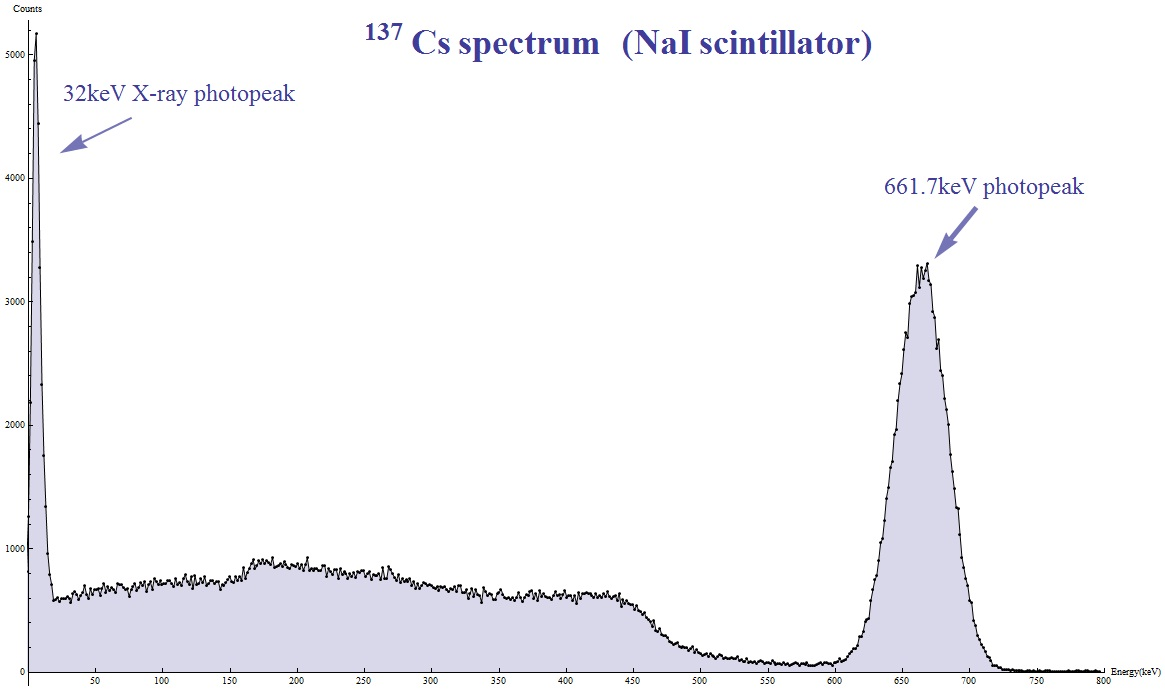
\includegraphics[width=\textwidth]{plots/csspektrum.JPG}
  \caption{Mithilfe eines NaI Szintillationsdetektors aufgenommenes Energiespektrum eines $\ce{^{137}Cs}$ Gamma-Strahlers\cite{Caesium}}
  \label{fig:Spektrum}
\end{figure}
In der Abbildung ist bei $\SI{32}{\kilo\electronvolt}$ zusätzlich der durch Röntgenstrahlung\cite{rontgen} enstehende Photopeak zu sehen.\\
Wenn man die Frequez der Strahlung weiter erhöht, steigt ie Intensität der Strahlung wieder an, da die Photonen zu Cooper-Paaren zerfallen, welche aus einem Elektron und einem Positron bestehen. Dieser Prozess ist allerdings nur möglich wenn das betreffende Photon eine Energie größer als die Summe der Ruhemassen der entstehenden Teilchen hat, welche je bei ca. $\SI{511}{\kilo\electronvolt}$ liegt.
\subsection{Tomographie mittels Gamma-Strahlung}
\label{sub:tomo}
Bei der Tomographie handelt es sich um ein Verfahren zur Struturbestimmung von Objekten durch Aufnahme von Querschnittsbildern. Das Verfahren wird vorrangig in der Medizin zur Untersuchung von menschlchem Gewebe eingesetzt und basiert auf der Erkennung kleiner Dichteunterschiede im betrachteten Objekt. Zur Untersuchung der Probe, wird diese mit \gamma-Strahlung durchstrahlt und die durch Absorption verringerte Intensität wird mittels eines Szintillationsdetektors gemessen. Die Intensität $N$ ändert sich dabei gemäß des Absorptionsgesetzes
\begin{equation}
  N(r) = I_0 \exp{(-\mu r)}
  \label{eqn:absorp}
\end{equation}
wobei \mu der Absorptionskoeffizient des Materials und r die Strecke auf der die Strahlung Absorbiert wird darstellt.\\
Die nachfolgend verwendete Probe besteht aus mehreren Würfeln $i$ der Dicke $d_i$, wodurch sich \eqref{eqn:absorp} zu
\begin{equation*}
  \sum_i \mu_i d_i = \log{\left(\frac{I_0}{N_j}\right)}
\end{equation*}
verändert. Die Ausgangsintensität der j-ten Projektion ist hierbei durch $N_j$ gegeben. Mit der Matrix $\symbf{A}$ zur Beschreibung der Würfelgeometrie, sowie den Vektoren
\begin{center}
  $\vec{\mu} = (\mu_1,...,\mu_9)^\symup{T}$ und\\
  $\vec{I} = \log{\left(\frac{I_0}{N_j}\right)}$
\end{center}
lässt sich ein lineares Gleichungssystem der Form
\begin{equation}
  \symbf{A} \vec{\mu} = \vec{I}
\end{equation}
aufstellen. Nimmt man nun mehr Projektionen auf, als Würfel in der Probe enthalten sind, so erhält man ein überbestimmtes Gleichungssystem aus dem man durch
\begin{equation}
  \vec{\mu} = \left(\symbf{A}^\symup{T}\symbf{A}\right)^{-1}\cdot\symbf{A}^T \vec{I}
  \label{eqn:mu}
\end{equation}
die Absorptionskoeffizienten ermittlen kann. Die zugehörigen Abweichungen werden nach
\begin{equation}
  \sigma_i = \sqrt{\text{diag}\{\left(\symbf{A}^\symup{T}\symbf{A}\right)^{-1}\}}
  \label{eqn:Fehler}
\end{equation}
berechnet. Diese Methode wird als Methode der kleinsten Quadrate bezeichnet.
